\chapter{Methodology}

This chapter takes an in-depth look at the methodology used in this project. It covers the way the data is obtained, the features used, and a discussion on what to consider a hit song. It also take a closer look at the data to see what can be learned just by analysing it on its own and how it needs to be prepared for the machine learning algorithms to work better. Finally, the evaluation measures are presented and the training and testing protocols are explained along with the optimisation of the hyperparameters of the models.

\section{Description of data sources}
Spotify \cite{kreitz2010spotify} is one of the largest music streaming services available today with about 200 million monthly active users. In 2014, Spotify bought Echo Nest \cite{SpotifyEchoAquisition:online} which was a music intelligence and data platform and along with it, it got a database of 30 million songs \cite{TheEchoN16:online} containing data aggregated from web crawling, data mining, and digital signal processing techniques. As seen in Section \ref{sec:relatedwork}, The Echo Nest API was a common source for data in related research in this area. It now powers Spotify's music recommendation and playlist curation features. It is worth mentioning that with it being such a popular streaming service nowadays, artists or record labels use it as one of their main distribution platforms and so upload the music to the service to release it to the world. Spotify also provides an API to query that database and get information about any song. 

The data used in this project was all made available by this freely available Spotify Web API \cite{WebAPI:online}. The API allows access to information about songs in their database such as song title, artist name, etc. but also contains a different endpoint to get information derived by their music intelligence algorithms. 

For each song that is added on their platform they store the usual metadata such as artist name, song title, release date, album cover, etc. but also calculate a range of audio features using signal processing and some proprietary algorithms. There are 13 such features and those are: duration, key, mode, time signature, acousticness, danceability, energy, instrumentalness, liveness, loudness, speechiness, valence and tempo. Some of these are direct features of the audio(such as duration) but others (such as dancebility) are calculated by Spotify and provide more abstract measures. A more in depth explanation of each of those features can be found in Table \ref{tab:feature}.
Since these features are calculated for every song in their database they can be used to compare the songs with each other and as input for the machine learning models.

To query the API a Python script was created with the \textit{spotipy} library \cite{Spotipy:online} (a lightweight Python library for the Spotify API) that really simplified the interaction. The database of songs is truly huge but the songs vary a lot in genre, year of release, popularity, language and we need a subset that is representative of listening trends nowadays. For this project it was important that the songs represent the current popularity trend so a playlist was manually created using the Spotify Desktop Application. This playlists aggregated the top 50 songs on Spotify from various countries (US, UK, Brazil, Romania, France, Germany, etc.) to account for different tastes in music in different regions and had 600 songs. For each song the metadata and the audio features described above are retrieved and stored in a csv file. The algorithm is presented in pseudocode in Algorithm \ref{alg1}.
\begin{algorithm}[caption={"Getting the data"}, label={alg1}]
begin
    foreach song in the playlist
        get song metadata from API
        get song audio features from API
        store the information as a new row
    end
    write data to csv
end
    
\end{algorithm}

\section{Establishing the ground truth}
\label{ground_truth}
One of the very important questions that had to be answered early on was what exactly is a hit song or what it is considered to be in this research. Looking at related work, there have been a few different ways of approaching at this. Some studies used charts like the ones from Official Charts Company \cite{herremans2014dance} or Billboard Top 100 \cite{reiman2018predicting} considering a song a hit if it appeared on these charts. Others used a "song hotttnesss" metric from The Echo Nest API that ranged from 0 to 100 and set a threshold to consider everything above 75 to be popular \cite{pham2016predicting}. This project uses a metric provided by the Spotify API called \textit{popularity}, similar to the "song hotttnesss". This is a score between 0 and 100 calculated by Spotify using the number of plays a song gets and how recent those plays are. So, a very popular song should have a score of 100 and an unknown song should have a score close to 0 but even if a song has a lot of plays but those plays are not recent it will score low. This is useful since it also provides an insight into what the current trend is.

I chose to consider every song with a popularity of 90 or more as popular (class 1) and everything below that threshold as not popular (class 0). This threshold was chosen since we want to distinguish the truly popular songs, the top 10 percent, from the rest since that represents a more useful prediction. A lower threshold also resulted, based on experimentation, in poorer results. Based on that threshold value, binary labels are added to the songs. After cleaning the data of duplicates and entries with invalid values the data set has 570 songs out of which 55 songs are labelled as popular and 515 are not popular.

\section{Data insights}
Before applying machine learning, it is useful to plot features against each other to see if any information can be gained from the data itself.

\begin{figure}[h]
    \centering
    \begin{minipage}{0.45\textwidth}
        \centering
        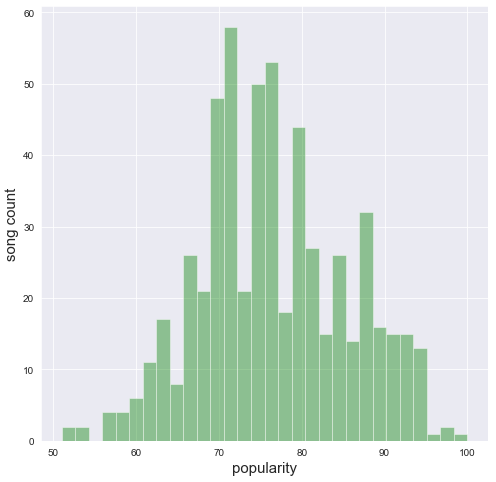
\includegraphics[width=0.9\textwidth]{methodology/fig/histogram.PNG} % first figure itself
        \caption{Popularity histogram}
        \label{fig:histo}
    \end{minipage}\hfill
    \begin{minipage}{0.45\textwidth}
        \centering
        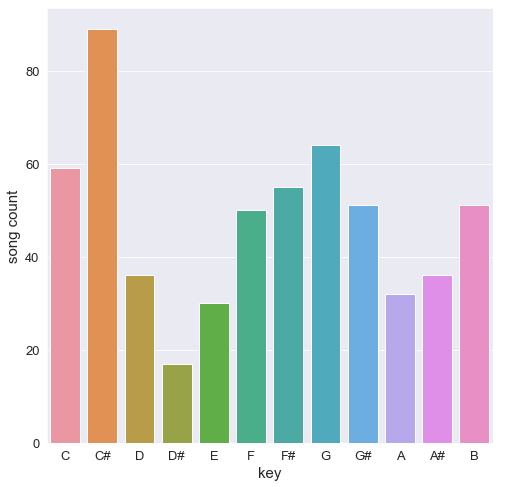
\includegraphics[width=0.9\textwidth]{methodology/fig/keycount.PNG} % second figure itself
        \caption{Key spread in data}
        \label{fig:keycount}
    \end{minipage}
    \begin{minipage}{0.45\textwidth}
        \centering
        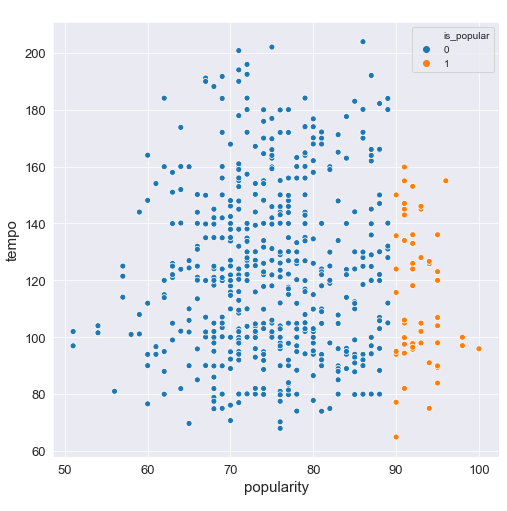
\includegraphics[width=0.9\textwidth]{methodology/fig/temppop2.PNG} % third figure itself
        \caption{Tempo and popularity}
        \label{fig:temppop}
    \end{minipage}\hfill
    \begin{minipage}{0.45\textwidth}
        \centering
        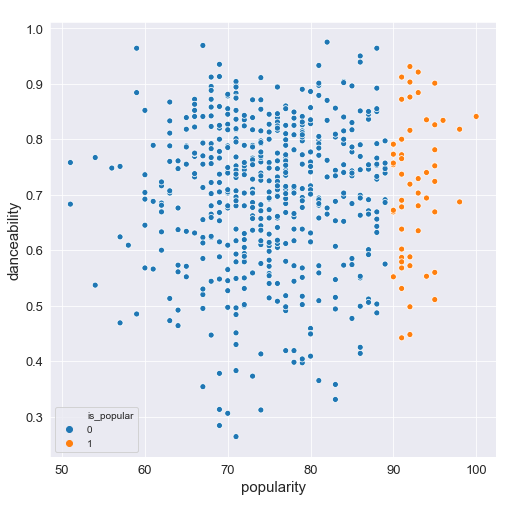
\includegraphics[width=0.9\textwidth]{methodology/fig/dancepop.PNG} % fourth figure itself
        \caption{Danceability and popularity}
        \label{fig:dancepop}
    \end{minipage}
\end{figure}

In Figure \ref{fig:histo} it can be observed that most of the songs in this data set lie in the 70 to 80 popularity range and in Figure \ref{fig:keycount} it can be seen that the keys C\# and G seem to be more common, while D\# is the least common. While there are no very distinct clusters, using Figure \ref{fig:temppop} and Figure \ref{fig:dancepop} some basic assumptions can be made such as if a song has a very high tempo or very low danceability it is likely not popular.

\section{Data pre-processing}
Before the data can be used in the machine learning algorithms it is important that it is scaled so that all the features are brought to the same level of magnitude. This is essential since some algorithms calculate the distance between points using Euclidean distance and each feature should contribute approximately proportionally to the final distance. Scaling is applied for all the features and each scaled feature value is calculated like in Equation \ref{eq:scaling}.

\begin{equation}
z\ =\ ( x\ -\ u) \ /\ s
\label{eq:scaling}
\end{equation}
\addvbuffer[12pt 8pt]{
\begin{tabular}{lll}
	where & $z$ & is the scaled feature value,\\
	& $x$ & is the feature value before scaling,\\
	& $u$ & is the mean of the feature,\\
	& $s$ & is the standard deviation of the feature.
\end{tabular}
}

In Figure \ref{fig:beforesca} and Figure \ref{fig:aftersca} the difference between non-scaled and scaled data can be observed. The data still has the same shape but the values on the y-axis are much smaller after scaling in Figure \ref{fig:aftersca}. The standard deviation and mean can also be calculated without transforming the data so that the transformation can be applied at a later point. This is useful since we might want to scale the test set separately but still apply the same transformation applied to the training data.

\begin{figure}[h]
    \centering
    \begin{minipage}{0.45\textwidth}
        \centering
        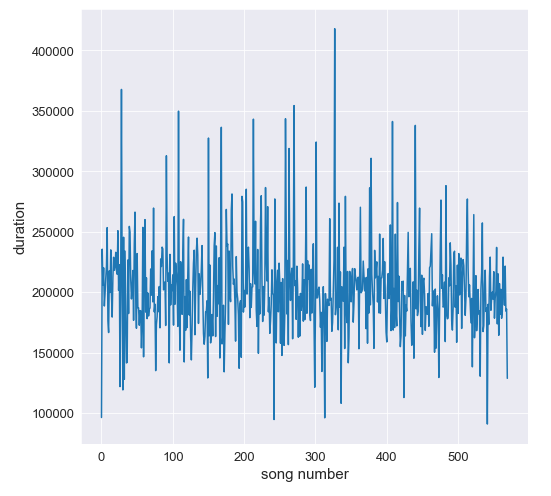
\includegraphics[width=0.9\textwidth]{methodology/fig/beforescaling.PNG} % first figure itself
        \caption{Duration before scaling}
        \label{fig:beforesca}
    \end{minipage}\hfill
    \begin{minipage}{0.45\textwidth}
        \centering
        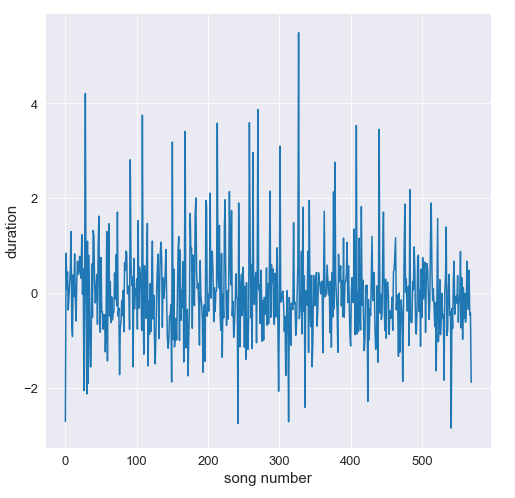
\includegraphics[width=0.86\textwidth]{methodology/fig/afterscaling.PNG} % second figure itself
        \caption{Duration after scaling}
        \label{fig:aftersca}
    \end{minipage}
\end{figure}

With the data scaled, it is now ready to be used by classification algorithms.

\section{Evaluation measures}
\label{sec:evalation}
Since accuracy can be misleading (as discussed in \autoref{sec:imbalance}), other metrics were also used to evaluate the models. Some metrics derived from the confusion matrix such as precision, recall, specificity and F1-score (a weighted average of precision and recall \cite{sklearnm18:online}) were inspected but mainly the Area Under the Receiver Operating Characteristic Curve (AUROC) \cite{bradley1997use} \cite{fawcett2006introduction} was used. The ROC curve represents the True Positive Rate plotted against the False Positive Rate for every possible classification threshold (also called the decision threshold - the value above which an example is considered to be of class 1 - 0.5 by default). The true positive rate is also called recall and it is a measure of how often the prediction is positive when the actual label is 1. The false positive rate is equal to 1 - specificity and it is a measure of how often the prediction is positive when the actual label is 0. The curve can also be seen as a plot of the hit rate versus the false alarm rate. A good classifier would have a curve that spans the upper left corner while a random predictor would have a curve that looks more like the identity line. An example of an ROC curve can be seen in Figure \ref{fig:rocsvm}. AUROC or simply AUC is a good way of measuring the performance of that classifier based on the ROC curve and it tells us how capable the model is of distinguishing between the two classes \cite{ROCAUC:online}. This is a better way of evaluating models because while accuracy only represents the score for one threshold this looks at all the possible thresholds. A good model will have an AUC score close to 1 meaning it is able to separate the two classes while a random predictor would have a score closer to 0.5.

\section{Training and testing protocols}

Since the classifiers have been picked, the next steps in the model selection process are the training and testing of the models. They need to be trained so they can learn and be tested so we can make sure that the pattern they have learned is indeed useful and does not only apply to the input data. That phenomenon is known as overfitting and it means that the model learns a rule that applies too tightly to the training set and will not work well in the real world. To reduce the chances of that happening, a technique known as cross validation is used. Cross validation splits the data set into equally sized chunks called folds. One fold will be left out for testing and the rest are used for training. This process is repeated until every fold has been used for both training and testing as shown in Figure \ref{fig:cv} for five folds. The cross validation strategy used in this project, shuffles the training examples and tries to ensure the same balance of classes in the folds (ten in this case) as in the whole data set \cite{SratifiedCv:online}. 

\begin{figure}[h]
\centering
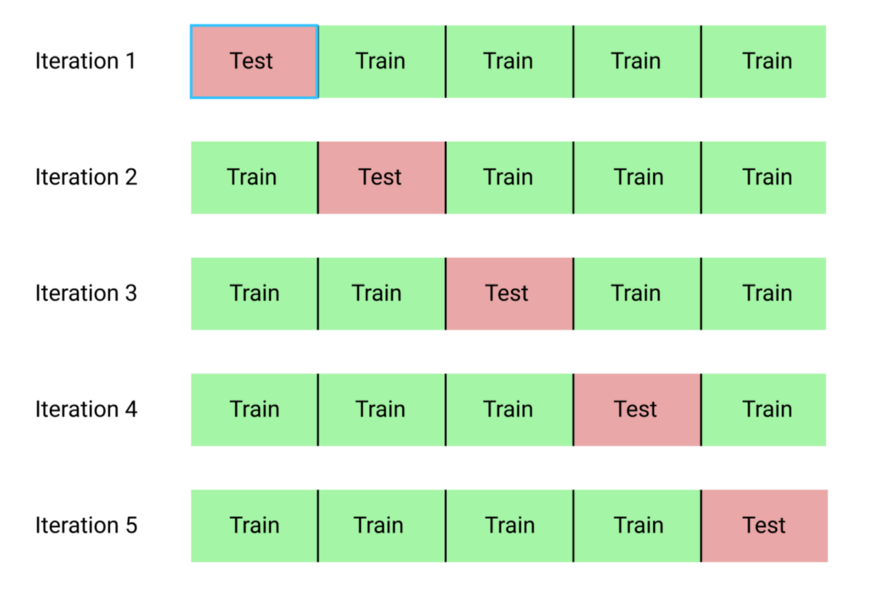
\includegraphics[width=0.7\linewidth]{methodology/fig/cv.png}
\caption{Cross validation process \cite{CrossVal24:online}}
\label{fig:cv}
\end{figure}

\begin{algorithm}[caption={"Model selection algorithm"}, label={alg2}]
begin
    foreach model in the model list
      do cross validation on model selection data set
        calculate score for each iteration
      end
      calculate average CV score for all iterations
      test model on world set
      calculate generalisation score
    end
    choose best model
end
    
\end{algorithm}



Before the cross validation process, the data set is first split into two sets. A bigger one for the cross validation (the model selection set in Figure \ref{fig:modelsel}) and a smaller one (the world set) that will be used for testing. To know how well the models will generalise, how well they will perform in the real world, the smaller subset of data will be kept unseen by the cross validation process to further test the models. That will give an additional indication of whether the models have overfitted the data or not. The whole process is visually described in Figure \ref{fig:modelsel} and algorithmically in pseudo-code in Algorithm \ref{alg2}.

\begin{figure}[h]
\centering
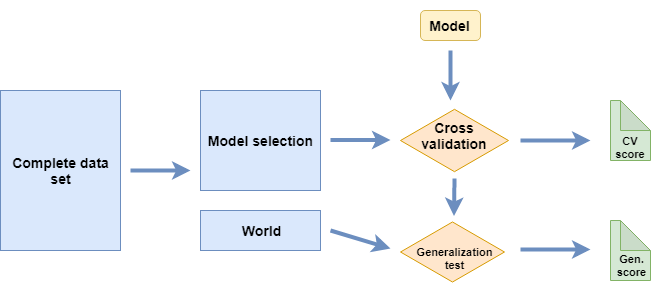
\includegraphics[width=0.9\linewidth]{methodology/fig/process.png}
\caption{Data split for model selection and process diagram \cite{CrossValVimeo:online}}
\label{fig:modelsel}
\end{figure}



\section{Hyperparameter optimisation}

To squeeze every little bit of performance out of the models we can look for the best parameters for the learning algorithms. To do so, Grid Search and cross validation are used. Grid search works similarly to the feature selection algorithm \ref{alg3}. A list of parameters and parameter values like in Figure \ref{fig:hyper} is provided for every model and the algorithm loops through all the possible combinations, calculating scores for each of them. After it is done the best scoring parameter combination is picked.

\begin{figure}[h]
\centering
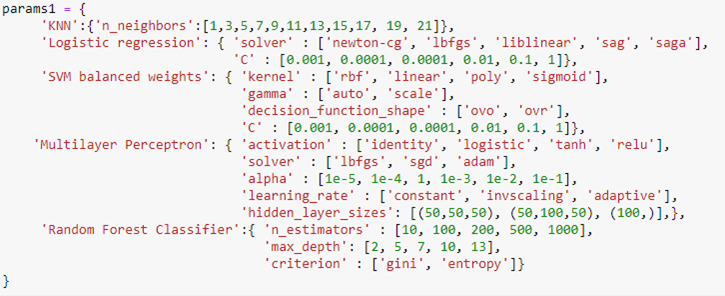
\includegraphics[width=0.9\linewidth]{methodology/fig/hyper.png}
\caption{Example of parameter lists provided for models to be used for Grid Search}
\label{fig:hyper}
\end{figure}

The features selected might influence the parameters chosen and the parameters might influence the features so ideally both of these operations should be done at the same time. This would greatly increase the computation time and might not even be feasible. In this project, a basic manual parameter optimisation was done before the feature selection process and the grid search algorithm was ran to fine tune those parameters on the chosen features after.

Some of the outcomes of this process on this data are, for example, that the best performing kernel for SVMs is the RBF kernel, the best solver for MLP and Logistic Regression is the lbfgs solver and the optimal number of estimators for the Random Forrest is 100.